\documentclass[a4paper,14pt]{article}
\usepackage[left=2cm,right=2cm, top=2cm,bottom=2cm, bindingoffset=0cm]{geometry}
\usepackage[T2A]{fontenc}
\usepackage[utf8]{inputenc}
\usepackage[english,russian]{babel}
\usepackage{amsmath,amsfonts,amssymb,amsthm,mathtools,graphicx}
\usepackage{fancybox,fancyhdr}
\usepackage{tabularx}
\usepackage{multirow}
\usepackage{bigstrut}
\usepackage{booktabs}
\usepackage{float}
\usepackage{xcolor}
\usepackage{array}
\usepackage{caption}

\DeclareGraphicsExtensions{.pdf,.png,.jpg}

\author{Ануфриев Андрей}
\title{Лабораторная работа № 3.07 \\ Изучение свойств ферромагнетика}
\date{01.04.2026}

\begin{document}

    \begin{figure}[h]
        \centering
        \begin{minipage}{0.45\linewidth}
            \centering
            
\includegraphics[width=\linewidth]{slogan_chernyy.png}
            \label{fig:slogan}
        \end{minipage}
        \hfill
        \begin{minipage}{0.45\linewidth}
            \centering
            
\includegraphics[width=\linewidth]{cs-logo.png}
            \label{fig:logo}
        \end{minipage}
    \end{figure}
    \begin{table}[htbp]
        \centering
        \begin{tabular}{lrlr}
            Группа & \qquad \qquad P3219 & К работе допущен & \qquad \qquad \qquad \qquad \qquad \qquad \\
            \cmidrule{2-2}\cmidrule{4-4}
            Студент &  \qquad \qquad Торопов П.К.  & Работа выполнена & \qquad \qquad \qquad \qquad \qquad \qquad \\
            \cmidrule{2-2}\cmidrule{4-4}
            Преподаватель & \qquad \qquad Коробков М.П. & Отчет принят & \qquad \qquad \qquad \qquad \qquad \qquad \\
            \cmidrule{2-2}\cmidrule{4-4}
        \end{tabular}%
    \end{table}%
    \vspace{2cm}
    \begin{center}
        \LARGE
        Отчет по лабораторной работе № 3.07 \\
        Изучение свойств ферромагнетика

    \end{center}
    \vspace{13cm}
    \begin{center}
        2026 год
    \end{center}
    \newpage

% ===== ЦЕЛИ =====
\section{Цели работы}

\begin{enumerate}
    \item Измерение зависимости магнитной индукции в ферромагнетике от напряженности магнитного поля $B = B(H)$.
    \item Определение по предельной петле гистерезиса индукции насыщения, остаточной индукции и коэрцитивной силы.
    \item Получение зависимости магнитной проницаемости от напряженности магнитного поля $\mu = \mu(H)$ и оценка максимального значения величины магнитной проницаемости.
    \item Расчет мощности потерь энергии в ферромагнетике в процессе его перемагничивания.
\end{enumerate}

% ===== РАБОЧИЕ ФОРМУЛЫ =====
\section{Рабочие формулы и теоретические сведения}

Индукция магнитного поля в ферромагнетике:
\begin{equation}
    \vec{B} = \mu_0(\vec{H} + \vec{J}),
    \label{eq:induction}
\end{equation}
где $\vec{H}$ — напряженность магнитного поля, $\vec{J}$ — намагниченность, $\mu_0 = 4\pi \times 10^{-7}$\,Гн/м.

Магнитная проницаемость:
\begin{equation}
    \mu = 1 + \frac{J}{H} = \frac{B}{\mu_0 H}.
    \label{eq:permeability}
\end{equation}

Напряженность магнитного поля в катушке:
\begin{equation}
    H = \alpha K_x X,
    \label{eq:H}
\end{equation}
где $\alpha$ — масштабирующий коэффициент, $K_x$ — цена деления по оси X, $X$ — координата на экране.

Магнитная индукция:
\begin{equation}
    B = \beta K_y Y,
    \label{eq:B}
\end{equation}
где $\beta$ — масштабирующий коэффициент, $K_y$ — цена деления по оси Y, $Y$ — координата на экране.

Мощность потерь энергии при перемагничивании:
\begin{equation}
    P = \chi S_{\text{ПГ}},
    \label{eq:power}
\end{equation}
где $S_{\text{ПГ}}$ — площадь петли гистерезиса (в делениях экрана), а коэффициент
\begin{equation}
    \chi = K_xK_y\frac{N_1R_2C_1}{N_2R_1}f.
    \label{eq:chi}
\end{equation}

% ===== ИЗМЕРИТЕЛЬНЫЕ ПРИБОРЫ =====
\section{Измерительные приборы и установка}

Лабораторная установка состоит из:
\begin{itemize}
    \item Сердечника (магнитопровода) трансформатора с прямоугольным поперечным сечением;
    \item Генератора синусоидального напряжения АКИП-3409/2 (диапазон частот 20--40 Гц);
    \item Цифрового запоминающего осциллографа GDS-71102B для наблюдения петли гистерезиса в режиме XY;
    \item Первичной обмотки с $N_1$ витками;
    \item Вторичной обмотки с $N_2$ витками;
    \item Интегрирующей RC-цепочки для определения магнитной индукции.
\end{itemize}

Параметры установки и магнитопровода:
\begin{itemize}
    \item Сопротивление первичной обмотки: $R_1 = 68$\,Ом;
    \item Сопротивление вторичной обмотки: $R_2 = 470000$\,Ом;
    \item Емкость конденсатора: $C_1 = 4{,}7 \times 10^{-7}$\,Ф;
    \item Площадь поперечного сечения: $S = 0{,}000067$\,м$^2$;
    \item Средняя длина магнитопровода: $\ell = 0{,}078$\,м;
    \item Число витков первичной обмотки: $N_1 = 1665$;
    \item Число витков вторичной обмотки: $N_2 = 970$.
\end{itemize}

Калибровочные коэффициенты:
\[
    \alpha = 313{,}914\ \text{А/(м·мВ)}, \quad \beta = 3{,}399\ \text{Тл/(В·мВ)}, \quad \pi = 3{,}141593.
\]

Дополнительные параметры $K_x$ и $K_y$ (цена деления по осям X и Y) записывались из элементов управления осциллографа для каждого измерения.

% ===== РЕЗУЛЬТАТЫ ИЗМЕРЕНИЙ =====
\section{Результаты прямых измерений и расчёт зависимостей}

Совокупность результатов 38 измерений в диапазоне напряженности 0.35--96.7 А/м приведена в таблице~\ref{tab:measurements}. Измерения проведены при различных амплитудах выходного напряжения генератора.

\begin{table}[H]
\centering
\caption{Результаты измерений и расчётные величины для кривой начального намагничивания (часть 1)}
\label{tab:measurements}
\small
\begin{tabular}{|c|c|c|c|c|c|}
\hline
№ & $U$, В & $H$, А/м & $B$, Тл & $\mu$ & Примечание \\
\hline
1   & 19.0 & 96.69  & 0.1278 & 1052  & Максимум B \\
2   & 18.5 & 89.15  & 0.1258 & 1123  & \\
3   & 18.0 & 77.85  & 0.1230 & 1258  & \\
4   & 17.5 & 74.71  & 0.1196 & 1274  & \\
5   & 17.0 & 74.08  & 0.1169 & 1256  & \\
6   & 16.5 & 72.83  & 0.1142 & 1248  & \\
7   & 16.0 & 67.81  & 0.1115 & 1308  & \\
8   & 15.5 & 64.04  & 0.1081 & 1343  & \\
9   & 15.0 & 59.77  & 0.1033 & 1376  & \\
10  & 14.5 & 56.82  & 0.1006 & 1409  & \\
11  & 14.0 & 53.05  & 0.0952 & 1428  & \\
12  & 13.5 & 50.23  & 0.0925 & 1465  & \\
13  & 13.0 & 47.09  & 0.0908 & 1534  & \\
14  & 12.5 & 44.45  & 0.0870 & 1558  & \\
15  & 12.0 & 42.06  & 0.0816 & 1543  & \\
16  & 11.5 & 39.24  & 0.0789 & 1599  & \\
17  & 11.0 & 36.73  & 0.0765 & 1657  & \\
18  & 10.5 & 34.84  & 0.0734 & 1677  & \\
19  & 10.0 & 32.14  & 0.0693 & 1717  & \\
20  &  9.5 & 30.14  & 0.0666 & 1759  & \\
\hline
\end{tabular}
\end{table}

\begin{table}[H]
\centering
\caption{Результаты измерений и расчётные величины для кривой начального намагничивания (часть 2)}
\small
\begin{tabular}{|c|c|c|c|c|c|}
\hline
№ & $U$, В & $H$, А/м & $B$, Тл & $\mu$ & Примечание \\
\hline
21  &  9.0 & 28.13  & 0.0625 & 1769  & \\
22  &  8.5 & 26.37  & 0.0581 & 1754  & \\
23  &  8.0 & 11.36  & 0.0272 & 1904  & \\
24  &  7.5 & 10.45  & 0.0258 & 1967  & \\
25  &  7.0 &  9.67  & 0.0238 & 1958  & \\
26  &  6.5 &  8.92  & 0.0221 & 1972  & \\
27  &  6.0 &  8.04  & 0.0207 & 2053  & \textbf{Максимум $\mu$} \\
28  &  5.5 &  7.53  & 0.0187 & 1975  & \\
29  &  5.0 &  6.78  & 0.0170 & 1995  & \\
30  &  4.5 &  6.15  & 0.0156 & 2022  & \\
31  &  4.0 &  2.83  & 0.0054 & 1532  & \\
32  &  3.5 &  2.54  & 0.0046 & 1447  & \\
33  &  3.0 &  2.26  & 0.0041 & 1436  & \\
34  &  2.5 &  1.98  & 0.0037 & 1504  & \\
35  &  2.0 &  1.73  & 0.0034 & 1567  & \\
36  &  1.5 &  0.57  & 0.0014 & 1894  & \\
37  &  1.0 &  0.44  & 0.0006 & 1108  & \\
38  &  0.5 &  0.35  & 0.0003 &  705  & Минимум (слабое поле) \\
\hline
\end{tabular}
\end{table}

\textit{Примечание:} Выполнено 38 измерений в диапазоне $U = 0{,}5$--$19$\,В. Максимальная индукция: $B_{\text{max}} = 0{,}128$\,Тл при $H = 96{,}7$\,А/м; максимальная проницаемость: $\mu_{\text{max}} = 2053$ при $H = 8{,}04$\,А/м.

% ===== БЛОК ВЫЧИСЛЕНИЙ =====
\subsection*{Основные расчётные соотношения}

Для каждого измерения по соотношениям (\ref{eq:H}) и (\ref{eq:B}) вычислены:
\[
    H_i = \alpha K_x X_i, \quad B_i = \beta K_y Y_i, \quad \mu_i = \frac{B_i}{\mu_0 H_i}.
\]

Калибровочные коэффициенты: $\alpha = 313{,}914$ А/(м·мВ), $\beta = 3{,}399$ Тл/(В·мВ), $\mu_0 = 4\pi \times 10^{-7}$\,Гн/м.

Диапазон варьирования параметров (минимум -- максимум):
\begin{itemize}
    \item $H$: 0.35 -- 96.69 А/м (кратность: 276)
    \item $B$: 0.0003 -- 0.1278 Тл
    \item $\mu$: 705 -- 2053
\end{itemize}

% ===== ОБРАБОТКА =====
\section{Обработка результатов}

\subsection{Графики зависимостей B(H) и $\mu$(H)}

На рис.~\ref{fig:bh_large} и рис.~\ref{fig:mu_large} для всех 38 измерений показаны:
\begin{itemize}
    \item экспериментальные точки с погрешностями (±2\% для $H$ и $B$, ±3\% для $\mu$);
    \item \textbf{линейная интерполяция} между соседними измеренными точками;
    \item \textbf{аппроксимация} физически осмысленными моделями.
\end{itemize}

Для кривой начального намагничивания после сравнения альтернатив выбрана модель насыщения:
\begin{equation}
    B(H) = B_s\left(1-e^{-H/H_0}\right).
\end{equation}

Для зависимости магнитной проницаемости наилучшей оказалась феноменологическая модель с максимумом:
\begin{equation}
    \mu(H) = \mu_{\infty} + A\,x\,e^{1-x}, \quad x=\frac{H}{H_p}.
\end{equation}

\begin{figure}[p]
\centering
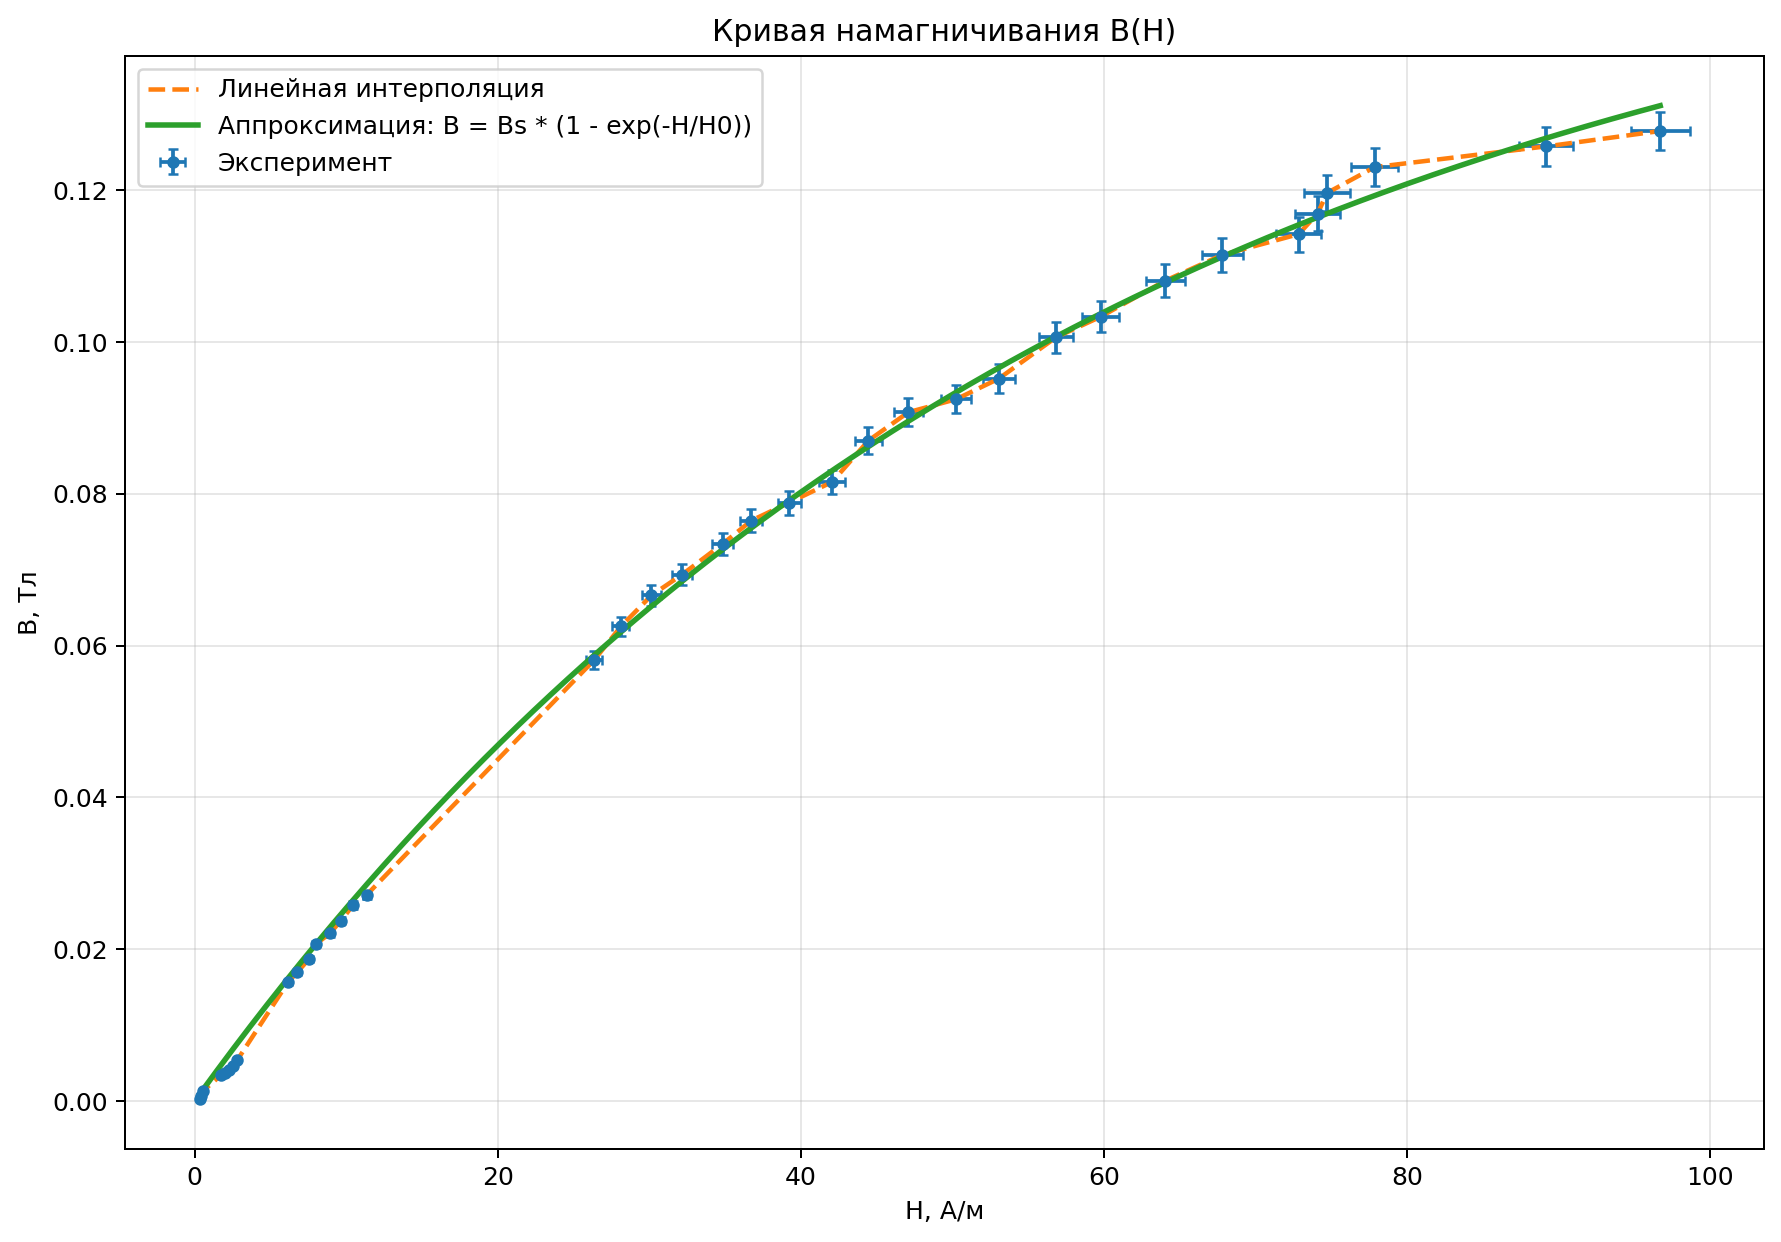
\includegraphics[width=\textwidth,height=0.88\textheight,keepaspectratio]{plot_bh_with_errors.png}
\caption{Кривая $B(H)$: экспериментальные точки, линейная интерполяция и аппроксимация}
\label{fig:bh_large}
\end{figure}

\begin{figure}[p]
\centering
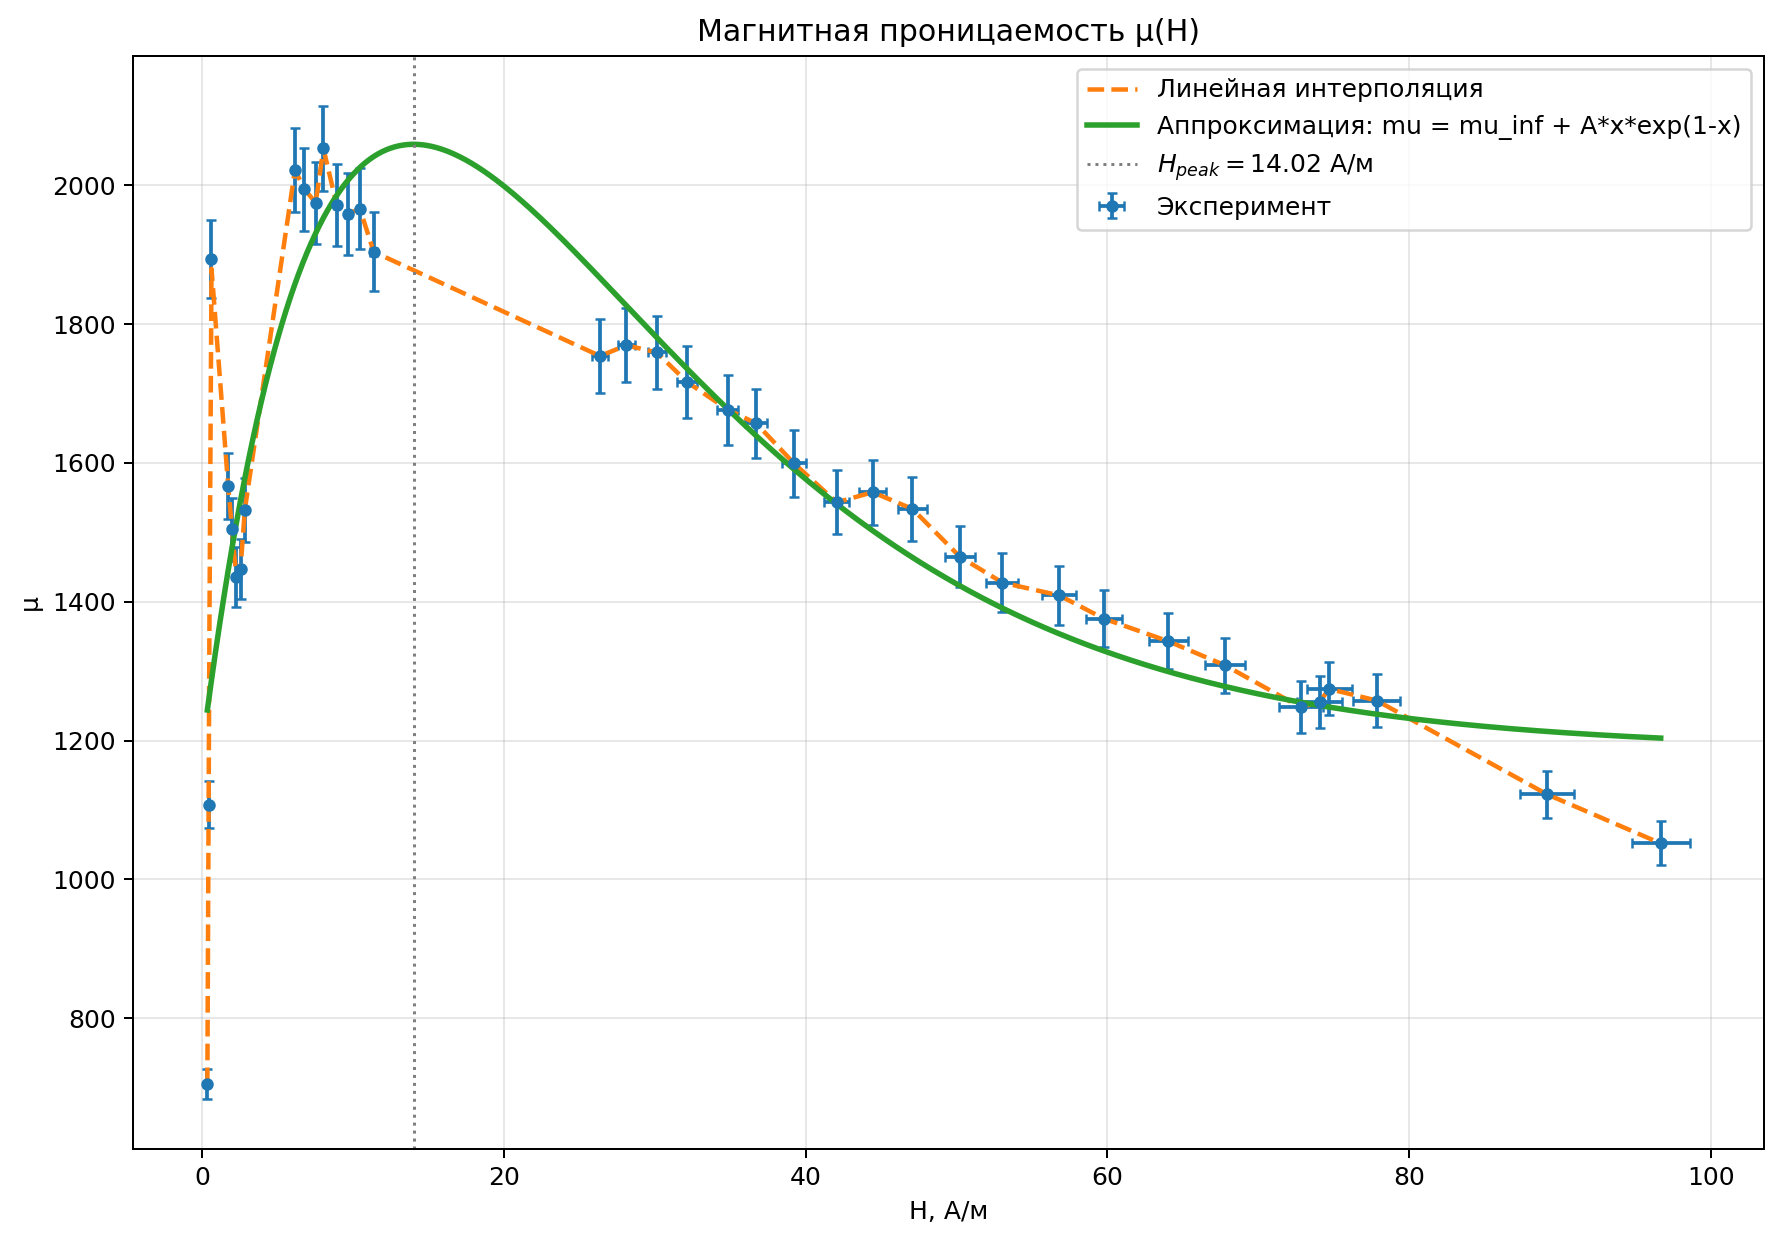
\includegraphics[width=\textwidth,height=0.88\textheight,keepaspectratio]{plot_mu_with_errors.png}
\caption{Кривая $\mu(H)$: экспериментальные точки, линейная интерполяция и аппроксимация}
\label{fig:mu_large}
\end{figure}

\clearpage

\subsection{Сравнение моделей, параметры и качество}

Параметры получены методом наименьших квадратов (скрипт \texttt{calculate\_results.py}):
\begin{itemize}
    \item для $B(H)$: $B_s = 0{,}1625$ Тл, $H_0 = 58{,}76$ А/м;
    \item для $\mu(H)$: $\mu_{\infty}=1187$, $A=872$, $H_p=14{,}02$ А/м,
    $\mu_{\max}^{\text{fit}}\approx 2059$.
\end{itemize}

В работе протестированы альтернативные аппроксимации и выполнено сравнение по $R^2$, RMSE и AIC.

Для $B(H)$ сравнивались:
\begin{itemize}
    \item $B=B_s(1-e^{-H/H_0})$;
    \item $B=B_s\tanh(H/H_0)$;
    \item $B=B_s\,H/(H+H_0)$.
\end{itemize}
Лучшая модель: $B=B_s(1-e^{-H/H_0})$ ($R^2=0{,}9990$, RMSE$=1{,}38\times 10^{-3}$ Тл, AIC$=-496{,}30$).

Для $\mu(H)$ сравнивались:
\begin{itemize}
    \item $\mu=\mu_{\infty}+Axe^{1-x}$;
    \item логнормальная пиковая модель;
    \item лоренцева пиковая модель.
\end{itemize}
Лучшая модель: $\mu=\mu_{\infty}+Axe^{1-x}$ ($R^2=0{,}765$, RMSE$=151$, AIC$=387{,}30$).

Качество выбранных аппроксимаций:
\begin{itemize}
    \item $B(H)$: $R^2 = 0{,}9990$, $\mathrm{RMSE}=1{,}38\times10^{-3}$ Тл;
    \item $\mu(H)$: $R^2 = 0{,}765$, $\mathrm{RMSE}=151$.
\end{itemize}

Более низкий $R^2$ для $\mu(H)$ связан с большим относительным разбросом в области слабых полей и сменой масштабов измерений, что характерно для расчётной величины $\mu = B/(\mu_0H)$.

\subsection{Характерные особенности кривых}

\textbf{Кривая B(H):} На участке $H < 10$\,А/м индукция возрастает резко (максимум проницаемости); при $H > 70$\,А/м наблюдается выход к насыщению.

\textbf{Кривая $\mu$(H):} Экспериментальный максимум $\mu_{\max} = 2053$ достигается при $H = 8{,}04$\,А/м. Аппроксимация воспроизводит максимум ($\mu_{\max}^{\text{fit}}\approx2059$) и тренд последующего снижения к области насыщения.

% ===== ИТОГОВЫЕ РЕЗУЛЬТАТЫ =====
\section{Итоговые результаты}

\subsection*{Основные характеристики материала}

\begin{table}[H]
\centering
\small
\begin{tabular}{|l|c|}
\hline
Параметр & Значение \\
\hline
Магнитная индукция (экспериментальный максимум) & $B_{\max} = 0{,}1278$ Тл \\
Магнитная индукция насыщения (по аппроксимации) & $B_s = 0{,}1625$ Тл \\
Максимальная проницаемость (эксп.) & $\mu_{\max} = 2053$ \\
Поле при максимуме проницаемости (эксп.) & $H_{\max\mu} = 8{,}04$ А/м \\
Поле максимума проницаемости (fit) & $H_p = 14{,}02$ А/м \\
Диапазон исследованных полей & $0{,}35$--$96{,}69$ А/м \\
Кратность диапазона & 276 \\
\hline
\end{tabular}
\end{table}

% ===== ИДЕНТИФИКАЦИЯ =====
\section{Идентификация материала образца}

По совокупности параметров ($\mu_{\max}\approx2053$, экспериментальный максимум $B_{\max}=0{,}1278$ Тл, модельное насыщение $B_s\approx0{,}1625$ Тл) исследуемый образец соответствует мягкому ферромагнитному материалу, характерному для трансформаторной (электротехнической) стали.

% ===== ВЫВОДЫ =====
\section{Выводы}

\begin{enumerate}
    \item По 38 экспериментальным точкам построены зависимости $B(H)$ и $\mu(H)$ в диапазоне $H=0{,}35$--$96{,}69$ А/м. Кривая $B(H)$ демонстрирует нелинейный рост и переход к насыщению.

    \item Для обработки данных использованы линейная интерполяция и аппроксимация; модели сравнивались по $R^2$, RMSE и AIC:
    \begin{itemize}
        \item для $B(H)$ лучшая модель: $B(H)=B_s(1-e^{-H/H_0})$, $R^2=0{,}9990$;
        \item для $\mu(H)$ лучшая модель: $\mu(H)=\mu_{\infty}+Axe^{1-x}$, $R^2=0{,}765$.
    \end{itemize}

    \item Определены ключевые характеристики материала: $B_{\max}=0{,}1278$ Тл, $B_s=0{,}1625$ Тл (по fit), $\mu_{\max}=2053$ при $H=8{,}04$ А/м.

    \item Полученные значения и форма кривых соответствуют мягкому ферромагнетику и согласуются с физическим смыслом процессов намагничивания (рост доменной подвижности в слабых полях и снижение эффективной проницаемости при приближении к насыщению).

    \item В текущей версии отчета основной акцент сделан на начальной кривой намагничивания и зависимости $\mu(H)$; параметры предельной петли ($B_r$, $H_c$) и оценка мощности потерь $P$ в этот объем обработки не включались.
\end{enumerate}

\end{document}

